\subsection{General Overview On Machine Learning}
\label{sub:GeneralML}
This section serves as a summary of general machine learning concepts
which are recommended to better understand the rest of the report.
The theory originates mainly from the machine learning course\cite{learningfromdata2012course} and the accompanying text book\cite{learningfromdata2012book}.

\subsubsection{Types of Machine Learning}
\label{ssub:TypesofMachineLearning}
As mentioned in the \nameref{sec:Introduction} (see Section~\ref{sec:Introduction}),
machine learning is a way of picking a fitting set of data to train on and calculate a model, 
such that similar data can be evaluated using the same model with high accuracy.
Generally speaking there are three popular types of machine learning:
supervised learning, reinforcement learning and unsupervised learning.
The type of learning is often for a project is often chosen on different sets criteria such as the type of data available,
and the knowledge about how the data is grouped.
More often than not the choice will lie on one single solution, something which will become clear in the following paragraphs.

\paragraph{Supervised Learning}
\label{par:SupervisedLearning}
To use supervised learning, the sample dataset used for learning must not only contain some valid input, but also the corresponding ``correct'' output.
The challenge therefore primarily lies on finding the right way of grouping or evaluating the input
such that the corresponding desired output can be achieved, by calculation on the model.
In many ways, this often makes Supervised Learning the most desired method, as there it is often easier to find a fitting solution which corresponds to what is observed on real-world data,
than when the desired output is completely unknown. It is also why, supervised learning has the most different techniques such as linear classification and support vector machines (see Section~\ref{ssub:ModelsforClassification}).

\paragraph{Reinforcement Learning}
\label{par:ReinforcementLearning}
Reinforcement learning is in many ways similar to supervised learning in that it requires both input data and corresponding output to be used.
The main difference is that while supervised learning requires the desired output to be correct, reinforcement only requires a grading of such output.
This technique is therefore often used, when there is no holistic overview regarding the distribution of data but where machine learning is till required.
\begin{exm}
Imagine a hospital where data is gathered on persons with an epidemical illness with multiple stages, and the
medical personnel would want to determine what factors could be causing such illness. As symptoms often can be misinterpreted on early stages,
it is unknown if the outcome is entirely correct but a grading of how ill a patient is can be used to aid the algorithm.
\end{exm}
In many ways reinforcement learning, also has to handle the grading additionally to finding a fitting model. 
This usually makes the models more complex, and as such harder to generalize properly\cite{sutton96generalizationin}\cite{boyan95generalizationin}.

\paragraph{Unsupervised Learning}
\label{par:UnsupervisedLearning}
The last popular type of learning is unsupervised learning, where only data input is given.
In many ways unsupervised learning tries to find a natural grouping or clustering of data,
such that input data that lies next to each other is grouped similarly.
This can be useful to e.g. separate colours from images or to find patterns in given input for further post-processing.
While it maybe hard to find real-world data that groups in obvious ways, and even harder making it fit some desired output;
Unsupervised learning has one advantage, that generalization is free. This is because unsupervised relies solely on input-processing and does not change
any output metrics and as such the models that can be used to not have to conform to an output specification.
Examples of unsupervised learning methods are k-means clustering\cite{learningfromdata2012book}, nearest neighbours\cite{scikitlearn2012nearestneighbours} and PCA\cite{smith2002tutorial}(see Section~\ref{sub:PCA} - \nameref{sub:PCA} for further explanation).

\paragraph{Selected Types of Learning}
\label{par:SelectedTypesofLearning}
To reduce the input space in our project, we resort to the use of PCA, which is as previously mentioned an unsupervised learning technique
and thus have no generalization cost. This allows us both to visualize how the variation/data is grouped, and allows us to
use supervised learning techniques to do the actual separation of data with much less noise and more performance than otherwise.
The choice of supervised learning is due to the fact that it offers the best trade-off between usefulness of output and generalization cost.

\subsubsection{Models for Classification}
\label{ssub:ModelsforClassification}
To be able to classify the resulting data from our experiments, we have chosen some simple supervised machine learning models to apply.
In the following sections we will thus present an overview of these models.
\paragraph{Linear Classification}
\label{par:LinearClassification}
The simplest type of classification is called linear classification.
The idea is simple: given an input dataset $\mathbf{X}$ consisting of data-vectors $\mathbf{x}$ with input parameters $x_1, \dots, x_n \in \mathbf{x}$ and the corresponding output parameter $y \in \left\{-1;+1\right\}$ (see Figure~\ref{fig:linearclass}), 
find a linear formula which separates the outputs given the input parameters.
The classes of output are usually denoted as either being negative (the output being $-1$) or positive (the output being $+1$). 
This makes it easier to run algorithms and is usually not a problem, because it is often possible to do a mapping from any given output format.\\

\begin{minipage}{\linewidth}
\centering
\makebox[\linewidth] {
  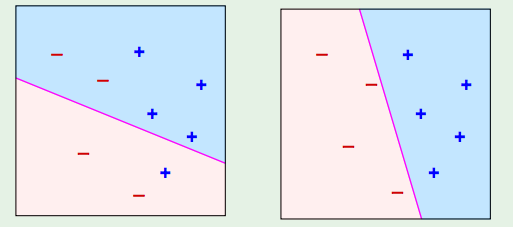
\includegraphics[width=0.5\textwidth]{LinearClassification.png}
}
\captionof{figure}{Linear classification algorithm running on two dimensional linear separable data}\label{fig:linearclass}
\end{minipage}\\\\

To separate the two classes of output, a given linear learning algorithm must assign weight coefficients to each input parameter.
To get a positive or negative classification out of the real-numbered output, the sign of the output is taken yielding two output classes.
The equation to be calculated therefore looks as follows:
$$ h(x) = sign\left(w_0 + w_1 \cdot x_1 + \dots + w_n \cdot x_n \right) $$
In order to allow separation of data with non-zero threshold value, an additional learning parameter $w_0$ is added.
If an artificial parameter $x_0=1$ is added this can be rewritten as:
$$ h(x) = sign\left(\sum_{i=0}^n{w_i \cdot x_i}\right) $$

\begin{algorithm}
  \begin{algorithmic}[1]
    \Require $\mathbf{X}$ a matrix of size $n\times m$ containing training data
    \Require $\mathbf{y}$ a vector of size $n$ which contains target output for each row vector $\mathbf{x} \in \mathbf{X}$
    \Ensure $\mathbf{w}$ a vector of size $n+1$ containing all the weights for target linear model
    \Function{CalculateWeights}{$\mathbf{X}, \mathbf{y}$}
    \Let{$\mathbf{w}$}{$\mathbf{0}$}
    \Repeat
    \ForAll{rows $\mathbf{x_j} \in \mathbf{X}$} 
    \Let{$y_j'$}{\Call{Sign}{$\sum_{i=0}^{n}{w_i\cdot x_{j,i}}$}}
    \EndFor
    \Let{$M$}{\Call{Misclassified}{$\mathbf{X}, \mathbf{y}, \mathbf{y'}$}}
    \Let{$\left(\mathbf{x_{m}}, y_{m}\right)$}{\Call{Any}{M}}
    \Comment{$\mathbf{x_{m}} \in \mathbf{X} \bigwedge y_{m} \in \mathbf{y}$} 
    \Let{$\mathbf{w}$}{$\mathbf{w} + y_{m} \cdot \mathbf{x_{m}}$}
    \Until{\Call{Misclassified}{$\mathbf{X}, \mathbf{y}, \mathbf{y'}$} = $\emptyset$}
    \EndFunction
  \end{algorithmic}
  \caption{The Perceptron Learning Algorithm}\label{alg:perceptron}
\end{algorithm}

The simplest linear algorithm is called the Perceptron Learning Algorithm (see Algorithm~\ref{alg:perceptron}). 
The idea is that the algorithm iteratively tries to adjust the weights by picking a misclassified point, and moving the separation line
such that the point is correctly classified. 

While this is normally done until the algorithm converges (i.e. until there are no misclassified points),
this might be impossible if the data is not completely separable.
In those situtations either a desired error rate $\epsilon$ is used or a hard limit on the number of iterations.

Linear classifications algorithms are generally good because the numbers of learning parameters are few, and thus they generalize well.

\paragraph{Logistic Regression}
\label{par:LogisticRegression}
While linear classification algorithms are simple and effective they have one disadvantage that they put a hard limit on output,
i.e. an output point is either positive or negative.
This makes it hard to identify borderline points, i.e. points which are close to the separation line, from those who are clearly in the separable region.

If these points are of interest, one choice could be to use Logistic Regression.
Logistic Regression is a learning model that enforces a softer limit on output than classical output by using the logistic function
\footnote{The logistic function usually results in a value $y \in \left(0;1\right)$, though it is ordinarily not a problem as
this can easily be translated to a scale corresponding to $\left(-1;1\right)$}
$\theta(s) = \frac{e^s}{1+e^s}$ instead of the sign function.

In this way the result would be a bounded real number which instead of specifying which class a point belongs to, specifies the probability of a point belonging to a specific class.
As we will see in Section \ref{par:MulticlassClassification}, this can be useful to use in Multiclass Classification where multiple classification algorithms ``vote'' on a given point.
\paragraph{Support Vector Machines}
\label{par:SupportVectorMachines}

Support Vector Machines are a set of advanced models that allows classification at low cost on generalization.
Strictly speaking, they exploit the fact that while all data is important for the learning algorithm there 
are only few points namely the neighbouring ones, also called the support vectors, which can influence the placement of the separation line (see Figure~\ref{fig:svm}).

\begin{minipage}{\linewidth}
\centering
\makebox[\linewidth] {
  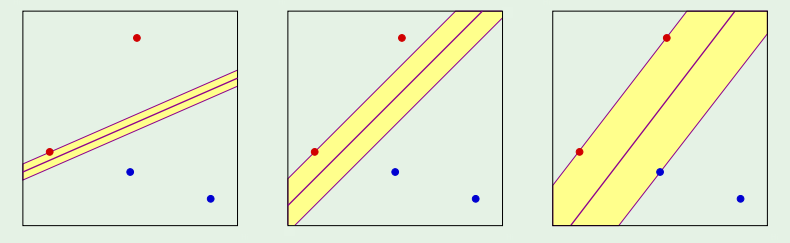
\includegraphics[width=0.5\textwidth]{SupportVectorMachines.png}
}
\captionof{figure}{Support Vector Machines - Maximizing the margin to the neighbouring points}\label{fig:svm}
\end{minipage}\\\\

While all correct separation lines has same generalization bounds, intuitively a separation line with larger margin to its neighbouring points seems more attractable.
This is due to the fact that a larger margin implies less possibility of misconfiguration of out-of-sample points; in other words it is easier for a data point to get
misclassified because it ``jumped'' over the separation line when the line is close, then when there is a considerable margin to it.
The goal of Support Vector Machine-based models is thus to maximize the distance between the separation line and its neighbouring points,
something which can be achieved with great performance using quadratic programming\cite{learningfromdata2012course}\cite{frank2006algorithm}. 
These properties make Support Vector Machines an excellent linear classifier, with generalization only dependent on the number of support vectors.

It should be noted that Support Vector Machines are also widely known for the ability
to allow non-linear transformation capabilities at low generalization cost via kernel methods. As these capabilities are not used in our project, we will not further
discuss those but the interested reader can refer to the "Learning From Data Course"\cite{learningfromdata2012course} for more information.

\paragraph{Multiclass Classification}
\label{par:MulticlassClassification}
In correlation with our experiment we have 4 lights which the test subjects are looking at, and as such we need to separate our data into 4 classes.
This means that in many ways classical classification is not enough if we want to have the full capabilities and therefore we have to resort to the use
of multiclass classification. While there are many approaches to multiclass classification,
two popular ways of doing multiclass classification are One versus One, and One versus Rest\cite{aly2005survey}\cite{scikitlearn2012multiclass}.
\begin{description}
  \item[One versus One] The idea of One versus One classification is to create $k$ binary classifiers for each $k$ classes,
    and then take a vote on each of the points such to see which classification the point fits best.
    While this is a novel approach it can perform competitively if the binary classifiers are used with a good learning model such as Support Vector Machines.
  \item[One versus Rest] In One versus Rest classification each pair of classes are compared on each point, and the class which compares favourably against the other classes
    wins the vote. While this creates a more complex and slower interaction, it usually performs better regarding classification than One versus One classification.
\end{description}

\subsubsection{Generalization}
\label{ssub:Generalization}
\paragraph{The Importance of Generalization}
\label{par:TheImportanceofGeneralization}
As mentioned in Section~\ref{sec:Introduction}, generalization is the concept on if it is possible to make the same assumptions on accuracy on training data,
as on the general data class. This concept is important because of the following observation, given a flexible enough model any data classification can be achieved
with almost complete accuracy on training data. That is we can always find a classification which fits the data, but that classification is seldom correct.
A learning model is only useful if it can be used in practice, and as we will see in Section~\ref{par:Bias-VarianceTrade-off} there is a correlation between model complexity
and its effect on generalization.
\paragraph{Bias -- Variance Trade-off}
\label{par:Bias-VarianceTrade-off}
One of the ways of measuring generalization capabilities of learning models are bias and variance. Bias-variance analysis depends on the mean learning function $\bar{g}$,
which represents the average separation function for a given dataset.
Bias is the measure of how well the mean learning function $\bar{g}$ approximates the target function $f$, i.e. the ability to generalize the learning model. Conversely,
variance is the measure of the probability of reaching the mean learning function $\bar{g}$, given any learning function $g$.
\begin{dfnt}
  \textbf{Bias} is the squared difference between the target function $f$ and the mean learning function $\bar{g}$ i.e. $\left(\bar{g}(x)-f(x)\right)^2$
\end{dfnt}
\begin{dfnt}
  \textbf{Variance} is the expected value of selecting a learning function $g$ close to the mean learning function $\bar{g}$ with a probability distribution on
  a dataset $D$ i.e. $\mathbb{E}_\mathcal{D}\left[(g^{(\mathcal{D})}(x)-\bar{g}(x))^2\right]$
\end{dfnt}

The correlation between and bias-variance analysis depends often on the dataset,
although it can generally be said that because simple models offer less flexibility they often do not track the target function well (i.e. they have a low variance),
while complex models can classify a complex dataset data more correctly, it is harder to reach the correct configuration (i.e. they have a low bias).

This results in a dilemma, choosing too simple of a model and it is possible to generalize the model well but with poor results, and choosing to
complex a model will make it hard to have good generalization but performs well on the training data.
This results in a trade-off where both the bias and variance must be kept sufficiently low to calculate a good learning model.
It is therefore necessary to chose the learning model based not only based on the appearance of the target data, but also on the number of data points available (see Figure~\ref{fig:biasvariance}).

\begin{minipage}{\linewidth}
\centering
\makebox[\linewidth] {
  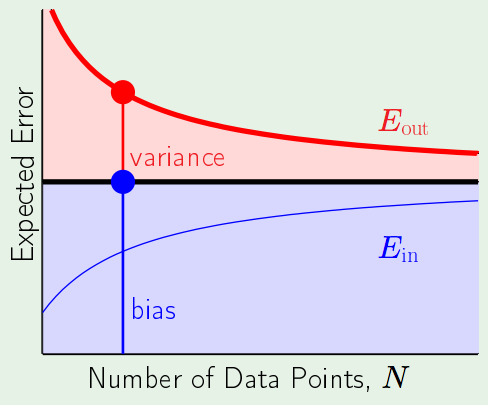
\includegraphics[width=0.5\textwidth]{BiasVariance.png}
}
\captionof{figure}{Bias -- Variance trade-off}\label{fig:biasvariance}
\end{minipage}

\subsubsection{Validation}
\label{ssub:Validation}
In Machine Learning Validation is a concept in which a part of the input data is reserved for calculating an error measure of a calculated model.
This can be useful in multiple scenarios such as  model selection and regularization.
\begin{description}
  \item[Model Selection] Validation allows calculating the accuracy of different learning models.
    While validation cannot be used exclusively to compare models because of inherent contamination\footnote{Validation data may be used in the training, and as such has an optimistic bias\cite{learningfromdata2012book}},
    it can be used as an aid for selecting good performing models and excluding models with bad accuracy.
  \item[Regularization] Validation metrics can be used to avoid overfitting.
    An overfitting model is a model which at cost of generalization performance, optimizes the model for the training data.
    This can be monitored by checking the validation score, and if the score worsens further training can be stopped i.e. the model is regularized.
\end{description}
\paragraph{Cross-Validation}
\label{par:Cross-Validation}
A common way of calculating a validation score, is by using cross-validation analysis. Cross-validation works by a dataset of size $n$ into $k$ chunks of data, and then
iterating through all $k$ chunks using them for validating a learning algorithm trained by the remaining $n-k$ chunks. 
By averaging the accuracy of the $k$ results, a more reliable metric can be given than a single validation instance due to the fact that there is a smaller probability of
partitioning the validation set in a ``lucky'' way.

As a rule of thumb $k=10$ provides a good validation score, while still being performing on large datasets\cite{learningfromdata2012course}.

\subsubsection{Testing}
\label{ssub:Testing}
Regardless of how performing a model is using the training data and how good a validation score it has,
testing using real-world data is important to truly determine its actual performance.

There are mainly two criterion for choosing a good test dataset: it must be a representative sample i.e. there must be enough data points to ensure that the testing is correct,
and it should be unbiased i.e. the test set must not have been used to train the model given.
Given these two conditions, it is possible to state that the test accuracy reflects the expected real-world accuracy.
This can be formalized by Hoeffding's inequality
$$\mathbb{P}\left[\left|\nu - \mu\right|> \epsilon\right]\leq 2\mathbf{e}^{-2\epsilon^2N}$$
which specifies that the probability of a sample probability $\nu$ tracking the general probability for error $\mu$ with accuracy $\epsilon$ is very small for large
number of data points $N$.
